In this section the five methods we have explained will be compared in term of performances, in addition also two other methods which have been explored during the lectures will be considered, SimCLR and BYOL. As we already said in the previous sections, the goal in SSL is having a good positive transfer in the downstream tasks, hence to compare the performances of the method we are going to see how using each one. In particular the considered downstream task will be image classification and object detection.

In table \ref{tab:imagenet-top1-5-acc-comp} we reported the top-1 and top-5 accuracy (the top-5 accuracy is available only for CPC and SimCLR) of the considered methods when tested for classification on the ImageNet dataset. All the methods uses as feature extractor a ResNet50.

\begin{table}[H]
	\centering
	\begin{tabular}{|l|l|cc|}
		\hline
		\multicolumn{1}{|c|}{\textbf{Method}} & \textbf{Architecture} & \multicolumn{2}{c|}{\textbf{ImageNet}} \\
		\multicolumn{1}{|c|}{} &  & Top1 & Top5 \\
		\hline
		Supervised & ResNet50 & 76.5 & - \\
		PIRL & ResNet50 & 63.6 & - \\
		CPCv2 & ResNet50 & 63.8 & 85.3 \\
		CMC & ResNet50  & 66.2 & 87 \\
		SimCLR & ResNet50 & 69.3 & 89.0 \\
		MoCov2 & ResNet50 & 71.1 & - \\
		BYOL & ResNet50  & 74.3 & 91.6 \\ 
		SwAV & ResNet50 & 75.3 & - \\
		\hline
\end{tabular}
	\caption{All architecture uses ResNet50}
	\label{tab:imagenet-top1-5-acc-comp}
\end{table}


\begin{table}[H]
	\centering
	\begin{tabular}{|l|l|cc|cc|}
		\hline
		\multicolumn{1}{|c|}{\textbf{Method}} & \textbf{Architecture} & \multicolumn{2}{c|}{\textbf{ImageNet 1\%}} & \multicolumn{2}{c|}{\textbf{ImageNet 10\%}} \\
		\multicolumn{1}{|c|}{} &  & Top1 & Top5 & Top1 & Top5  \\
		\hline
		Supervised & ResNet50 & 25.4 & 48.4 & 56.4 & 80.4 \\
		PIRL & ResNet50 & 30.7 & 57.2  & 60.4 & 83.8 \\
		SimCLR & ResNet50 & 48.3 & 75.5  & 65.6 & 87.8 \\
		BYOL & ResNet50  & 53.2 & 78.4  & 68.8 & 89.0 \\ 
		SwAV & ResNet50 & 53.9 & 78.5  & 70.2 & 89.9 \\
		CPCv2 & ResNet161 & - & 77.9 & - & 91.2 \\
		SimCLR & ResNet50 (4$\times$) & 63.0 & 85.8 & 74.4 & 92.6 \\
		BYOL & ResNet50 (2$\times$) & 71.2 & 77.7 & 89.5 & 93.7 \\
		\hline
	\end{tabular}
	\caption{Result after fine-tuning on 1\% of the data of ImageNet}
	\label{tab:imagenet-1-perc-semisup}
\end{table}


\begin{figure}[H]
	\centering
	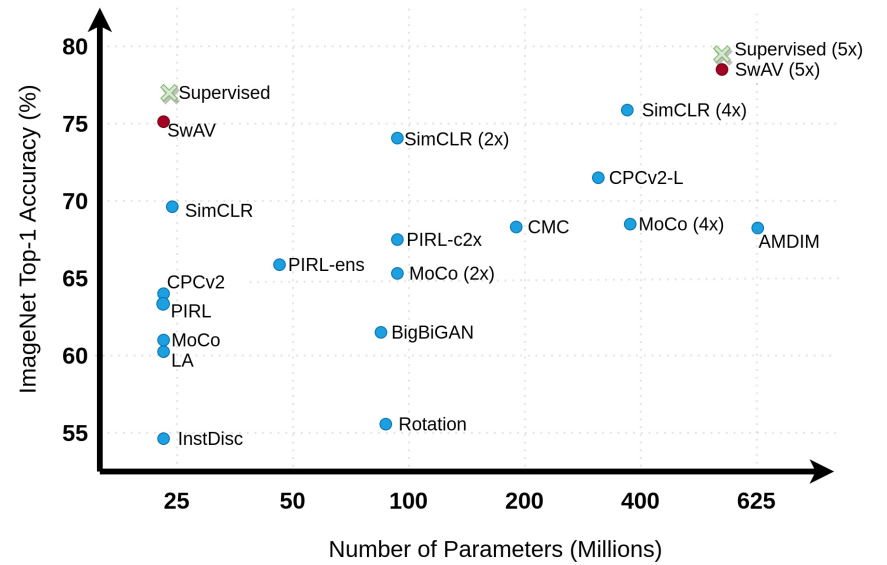
\includegraphics[width=10cm]{./images/imagenet-top1-acc-comp.png}
	\caption{Top-1 classification accuracy different contrastive learning methods with the number of parameters of the models}
	\label{fig:imagenet-top1-acc-comp}
\end{figure}